\documentclass[11pt]{article}

\usepackage{float}
\usepackage{hyperref}
\usepackage{graphicx}
\usepackage{amsmath}
% formatting
\usepackage{fullpage}
\usepackage{verbatim}
\usepackage{moreverb}
\usepackage{minted}
\usepackage{parskip}
\usepackage{hyperref}
\usepackage{multicol}
\let\verbatiminput=\verbatimtabinput
\def\verbatimtabsize{4\relax}
\newcommand{\repo}{fpga\_labs\_fa19}

\hypersetup{
  colorlinks=true,
  linkcolor=blue,
  urlcolor=blue
}

\begin{document}
\title{EECS 151/251A FPGA Lab\\
Lab 2: Introduction to FPGA Development + Creating a Tone Generator}

\author{Prof. Borivoje Nikolic and Prof. Sophia Shao \\
TAs: Cem Yalcin, Rebekah Zhao, Ryan Kaveh, Vignesh Iyer \\ Department of Electrical Engineering and Computer Sciences\\
College of Engineering, University of California, Berkeley}

\date{}
\maketitle

\section{Before You Start This Lab}

Make sure that you have gone through and completed the steps involved in Lab 1.
Let the TA know if you are not signed up for this class on Piazza or if you do not have a class account (eecs151-xxx), so we can get that sorted out.

To fetch the skeleton files for this lab, \texttt{cd} to the git repository (\texttt{\repo}) that you had cloned in the first lab and execute the command \texttt{git pull}.

You can find the documents/datasheets useful for this lab in the \texttt{\repo/resources} folder.
Go through the \href{http://inst.eecs.berkeley.edu/~eecs151/fa19/files/verilog/Verilog_Primer_Slides.pdf}{Verilog Primer Slides}; you should feel somewhat comfortable with the basics of Verilog to complete this lab.

\section{Our Development Platform - Xilinx Pynq-Z1}
For the labs in this class, we will be using the Xilinx Pynq-Z1 development board which is built on the Zynq development platform. Our development board is a printed circuit board that contains a Zynq-7000 FPGA along with a host of peripheral ICs and connections. The development board makes it easy to program the FPGA and allows us to experiment with different peripherals.

The best \href{https://reference.digilentinc.com/reference/programmable-logic/pynq-z1/reference-manual}{reference for this board} is provided by Digilent.
Browse the documentation there to get a feel for both what features the board has and, more importantly, what information the documentation has, should you need it later.

Being a development board, the silkscreen print clearly identifies connectors of interest. You should be able to recognize the most basic IO features on the board: GPIO LEDs, slide switches, and push-buttons. You should also be familiar with other basic elements of the board: input power socket, power switch, and the USB programming port. The following image identifies important parts of the board that may not have been obvious:

\begin{minipage}[h]{0.5\textwidth}
    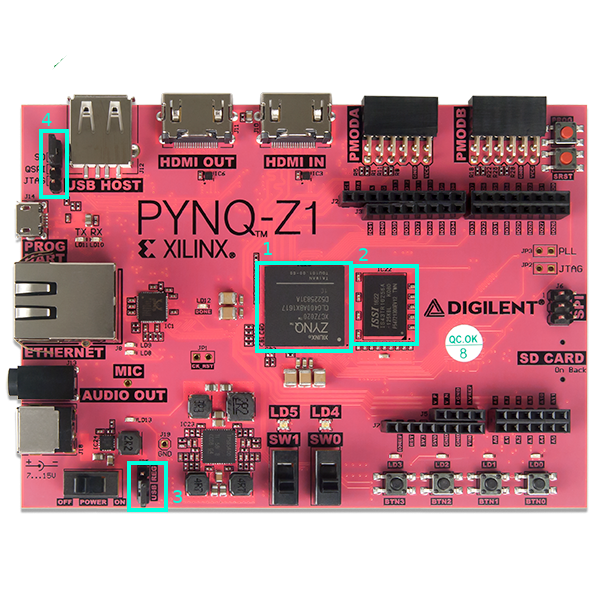
\includegraphics[width=\textwidth]{figs/z1_top_annotated.png}
\end{minipage}
\begin{minipage}[h]{0.5\textwidth}
    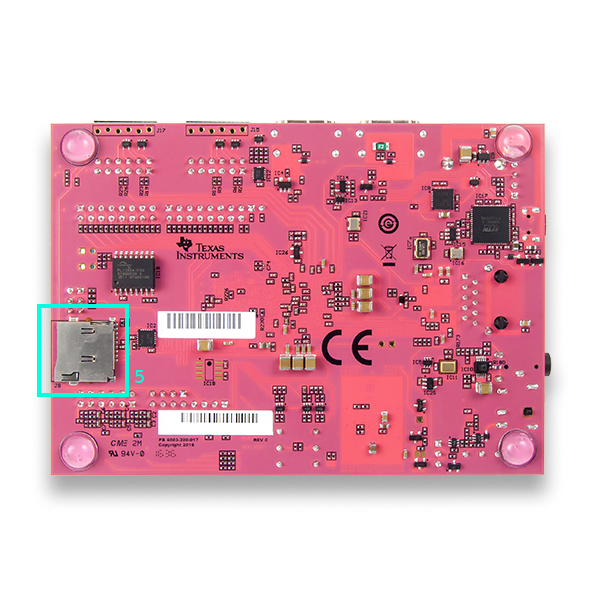
\includegraphics[width=\textwidth]{figs/z1_bottom_annotated.png}
\end{minipage}

\begin{enumerate}
  \item Zynq 7000-series FPGA. It is connected to the peripheral ICs and I/O connectors via PCB traces.
  \item ISSI DRAM chip
  \item Power source jumper: shorting "REG" has the board use the external power adapter as a power source; shorting "USB" has it rely on the 5 V provided by USB. The latter will work unless your design needs to power a lot of external peripherals. Since we have labs and power adaptors available, we avoid this.
  \item Programming mode jumper
  \item SD card slot
\end{enumerate}

\section{The FPGA - Xilinx Zynq-7000 7z020}
To help you become familiar with the FPGA that you will be working with through the semester, please skim Chapter 21: Programmable Logic Description of the \href{https://www.xilinx.com/support/documentation/user_guides/ug585-Zynq-7000-TRM.pdf}{Technical Reference Manual} and Chapter 2 of the \href{http://www.xilinx.com/support/documentation/user_guides/ug474_7Series_CLB.pdf}{Xilinx 7-series Configurable Logic Block User Guide}.
Pay particular attention to pages 15-25 on Slices and pages 40-42 on Multiplexers.
You will need to answer the following questions in your lab report (Section \ref{sec:labreport}).

\subsection{Lab Report Questions}\label{sec:checkoffQuestions}
\begin{enumerate}
  \item How many SLICEs are in a single CLB?
  \item How many inputs do each of the LUTs on a Zynq-7000 FPGA have?
  \item How many LUTs does the 7z020 have?
\item How do you implement logic functions of 7 inputs in a single SLICEL? How about 8? Draw a high-level circuit diagram to show how the implementation would look. Be specific about the elements (LUTs, muxes) that are used.
  \item What is the difference between a SLICEL and a SLICEM?
\end{enumerate}

\section{Overview of the FPGA Build Toolchain}
Before we begin the lab, we should familiarize ourselves with the CAD (computer aided design) tools that translate HDL (Verilog) into a working circuit on the FPGA.
These tools will pass your design through several stages, each one bringing it closer to a concrete implementation.
In previous years, older evaluation platforms (the ML505) used older FPGAs (a Xilinx Virtex-5 LX110T) and an older software suite (Xilinx ISE).
Although there was a GUI, we had Makefiles to invoke each subsequent program in the toolchain to carry out the complete synthesis and perform analysis.

Our new boards use Xilinx's updated design software, the Vivado Design Suite.
Vivado has integrated scripting capabilities (using the Tcl language) and integration with other high-level design tools (e.g. High-Level Synthesis).
The GUI itself has the disadvantage of being very manual to work with.
Repeatedly changing and running parameters quickly becomes tedious.
We will automate the design process after this lab, however, for learning, the GUI has the invaluable property of guiding us through each step of the process.
Read through the following sections but don't worry about the details for now.
We will run through the entire tool flow on a simple project at the end of this lab.

\subsection{Open the Lab 1 project in the Vivado Design Suite}
Now that you have cloned the \texttt{\repo} repository, you can \texttt{cd} to the \texttt{\repo/lab2} directory to see this lab's skeleton files.
You will note that there is a \verb|lab2.srcs| (sources) directory and a \verb|lab2.xpr| (project) file.

In our CentOS environment, press Alt-F2 to bring up a command dialog. Type the full path to the \texttt{vivado} binary to execute it:

\begin{verbatim}
/opt/Xilinx/Vivado/current/bin/vivado
\end{verbatim}

(You can also run this from a terminal or create a Desktop shortcut.)

Once in Vivado, open up the \texttt{lab2/lab2.xpr} project file. Look around the environment to try and get a feel for the GUI.

\subsection{Synthesis}
To run the synthesis step in the Vivado Design Suite (that is, turn your HDL into combinational and sequential logic), select \emph{Run Synthesis} in the \emph{Flow Navigator} pane to the left other interface. If this has been run before, the synthesized design can be inspected by selecting \emph{Open Synthesized Design}. Select \texttt{Schematic} under ``Open Synthsized Design" on the left toolbar to see a circuit schematic.

\subsection{Implementation}
The implementation step in the Vivado GUI is equivalent to the translation, mapping and place and route steps in the manual pipeline. Again, this takes the logical circuit synthesized previously and maps it to the physical logic devices our particular FPGA actually has. Select \emph{Run Implementation} in the \emph{Flow Navigator} to run it, then select \emph{Open Implementation} to inspect its outputs.

\subsection{Xilinx Design Constraints (XDC)}
How do we connect one of our signals to a physical device? How do we specify special properties of the circuit that might matter for correctness and timing?
The Xilinx Design Constraints file (with the \verb|.xdc| extension) specifies timing information and pin placement.
%XDC is inspired by the Synopsis ASIC synthesis toolchain and aims to be somewhat compatible. You are writing a form of TCL for the Vivado TCL interpreter.
More information can be found on page 22 of the \href{https://www.xilinx.com/support/documentation/sw_manuals/xilinx2015_2/ug911-vivado-migration.pdf}{Vivado migration guide}.

Take a look at this snippet from the XDC inside \verb|lab2/lab2.srcs/constrs_1/new/z1top.xdc|:
\begin{minted}{tcl}
set_property -dict { PACKAGE_PIN L19   IOSTANDARD LVCMOS33 } [get_ports { BUTTONS[3] }];
\end{minted}

This syntax assigns the properties \verb|PACKAGE_PIN| and \verb|IOSTANDARD| with the values \verb|L19| and \verb|LVCMOS33| (respectively) to the port \verb|BUTTONS[3]|, a signal we defined in our Verilog source. Each of these properties has a separate consequence in the synthesis process:

\begin{itemize}
\item The pin to which the \verb|BUTTONS[3]| signal should be connected to the physical pin L19 on the FPGA package.
\item The logic convention (maximum voltage, what ranges constitute low and high, etc) for that port will be LVCMOS33.
\end{itemize}

\subsection{Bitstream generation}
To generate the programming file our FPGA will understand, we invoke \emph{Generate Bitstream} in the \emph{Flow Navigator}.

\subsection{Timing Analysis}
A timing analysis report can be generated under \emph{Synthesis} in \emph{Flow Navigator}, by expanding \emph{Open Synthesized Design} and selecting \emph{Report Timing Summary}.

\subsection{Design Reports}
Reports are automatically generated at each step in the build flow. You should be able to discover them under each of the expanded stages in the \emph{Flow Navigator}. The \emph{Project Summary} window (under the \emph{Window} menu) presents a nice summary of the reports generated through each step. You will see some examples later in the lab.

\subsection{Programming the FPGA}
To send the bitstream to the FPGA with the Vivado GUI, we have to use the \emph{Hardware Manager}. This is accessible under \emph{Program and Debug} in the \emph{Flow Navigator}, right under \emph{Generate Bitstream}. Once connected to your FPGA over the USB JTAG interface, you can select \emph{Program Device} in the \emph{Flow Navigator} (or in the \emph{Hardware Manager} pane that opens) to perform the programming.

%\subsection{Toolchain Conclusion}
%This section was information dense. Don't worry about understanding the internals of each tool and the exact file formats they work with, especially for different Xilinx software generations. Just understand what each step of the toolchain does at a high level and you will be good for this class. You will use these kinds of tools regularly, but for now let the staff worry about making sure they work in the first place.

\section{Your First FPGA Design}
Finally, let's build a simple example of a complete project. Throughout the semester, you will build increasingly complex designs using Verilog, a widely used hardware description language (HDL). For this lab, you will use basic Verilog to describe a simple digital circuit.

Open up the \verb|lab2/lab2.srcs/sources_1/new/z1top.v| source file.
This file contains a Verilog module description which specifies which signals are inputs into the module and which signals are outputs.
Also check the constraints file in \verb|lab2/lab2.srcs/constrs_1/z1top.xdc|.

%Past versions of this course used an FPGA development toolchain from the Xilinx ISE Design Suite. The modern alternative, and that which we are now using for this course, is the Xilinx Vivado Design Suite (``Vivado'' for short). We will initially use Vivado's Integrated Development Environment (IDE) instead of any command-line tools, though you will eventually see that the framework (especially with Pynq) is ripe for automation with TCL and Python scripting.

%The lab skeleton files include the project meta data file, \verb|.xpr|, a Verilog source file for a simple top-level module, \verb|z1top.v|, and a constraints file, \verb|z1top.xdc|.

HDL source files like \verb|z1top.v| (where the HDL is Verilog) describe the circuit that you want to create on the FPGA.
\verb|z1top.v| describes a circuit that is the \emph{top-level} of your circuit: it has access to the signals that come into and out of the FPGA chip.
Constraints files, such as \verb|z1top.xdc|, allow the engineer (you!) to tailor specific properties of the synthesized design to how they wish to use their specific chip. This includes the crucial mapping between FPGA input/output pins and signal names used in circuit descriptions.

\subsection{Set up your Pynq-Z1}
\begin{enumerate}
  \item Plug in the power adaptor to provide mains power.
  \item Connect the USB interface to a spare USB port on your workstation.
  \item Turn the board on.
\end{enumerate}

The \verb|BUTTONS| input is a signal that is 4 bits wide (as indicated by the [3:0] width descriptor). This input signal represents the logic signals coming from the momentary push-button switches on the bottom right side of your Pynq-Z1 board. You should inspect your board to find these switches and confirm that there are 4 of them. Another basic input signal is \verb|SWITCHES|, which is 2 bits wide (as indicated by the [1:0] descriptor). Each of these two signals represents the slide switches on the Pynq-Z1, located just to the left of the momentary switches (look for SW0 and SW1).

The \verb|LEDS| output is a signal that is 6 bits wide (as indicated by the [5:0] width descriptor). This output signal represents the logic signals coming out of the FPGA and going into the bank of LEDs at the bottom right of the Pynq-Z1, just above the buttons. Almost. There are only 4 LEDs there; 2 more are tri-color LEDs located just above the slide switches in the middle.

In this file, we can describe how the slide switches, push buttons and LEDs are connected through the FPGA. There is one line of code that describes an AND gate that takes the values of one of the buttons and one of the slide switches, ANDs them together, and sends that signal out to the first LED. Let's put this digital circuit on the FPGA!

\subsection{Synthesize and Program}
\begin{enumerate}
  \item In Vivado, locate the \emph{Flow Navigator} pane to the left of the screen. Near the bottom, under \emph{Program and Debug}, click \emph{Generate Bitstream}. Accept the default settings and wait. This should invoke the dependent steps in the flow: \emph{Synthesis} and \emph{Implementation} (among other things).
    \begin{itemize}
      \item Selecting \emph{Project Manager} will give you a nice overview of the progress of various background steps while this happens.
      \item So will watching the \emph{Messages} and \emph{Logs} output.
    \end{itemize}
  \item When the synthesis and bitstream generation is done, select \emph{Open Hardware Manager} and connect to your FPGA.
    \begin{itemize}
      \item If you haven't before, or the hardware manager says no devices are connected, select \emph{Menu} $\rightarrow$ \emph{Open New Target}
      \item You should see \verb|xilinx_tcf| listed under Harware Targets in the top pane. In the bottom pane, two entries: \verb|arm_dap_0| and \verb|xc7z020_1|. That's good. \emph{Next} $\rightarrow$ \emph{Finish}.
    \end{itemize}
  \item Back in the \emph{Flow Navigator} on the left, under \emph{Program and Debug}, select \emph{Program Device}. The only option to program will be the FPGA, \verb|xc7z020_1|. The default bitstream file path should work too.
  \item See if it worked! What happens when you push the BTN0 button? What about when you change SW0? Both?
\end{enumerate}

\section{A Structural and Behavioral Adder Design and Inspecting the Schematic}
\subsection{Build a Structural 14-bit Adder}
To help you with this task, please refer to the `Code Generation with for-generate loops' slide in the Verilog Primer Slides (slide 35).

\begin{enumerate}
  \item Open \verb|lab2/lab2.srcs/sources_1/new/full_adder.v|; fill in the logic to produce the full adder outputs from the inputs
  \item Open \verb|structural_adder.v| and construct a ripple carry adder using the full adder cells you designed earlier and a `for-generate loop'.
  \item Inspect the \verb|z1top_adder.v| top-level module and see how your structural adder is instantiated and hooked up to the top-level signals.
    Look at the \verb|user_adder| instance of your structural adder.
    As we learned in previous lab, the basic I/O options on the Z1 board are limited. How are we managing to input two 3-bit integers?
  \item Set \texttt{z1top\_adder.v} as the top-level module by right-clicking \texttt{z1top\_adder} in Sources $\rightarrow$ Design Sources and click `Set as Top'.
  \item Run bitstream generation as usual
  \item Program the FPGA and test out the design; make sure you get correct results from your adder.
\end{enumerate}

%Run Synthesis, Implementation, and Generate the Bitstream for your design. (Remember that, in the GUI, you can select a later step in the pipeline and have all prerequisite steps performed automatically when prompted.) Program the board. Test out your design and see that you get the correct results from your adder. You should try entering different binary numbers into your adder with the switches and buttons and see that the correct sum is displayed on the GPIO LEDs.

If there are any problems with your design, you can view the output report in Vivado from the \emph{Project Summary} view. The Project Summary tab opens by default, but you can bring it up again from the \emph{Window} menu. See box 1 in the figure for an example. At the bottom of the screen (box 2 in the same figure) you can also inspect the outputs of the individual tools that make up the pipeline; there lies bountiful debugging information should you ever need it. Unfortunately, not every log or warning message is useful, but it will serve you well to compare what outputs you do see with the relative success you have with your design.

\begin{center}
  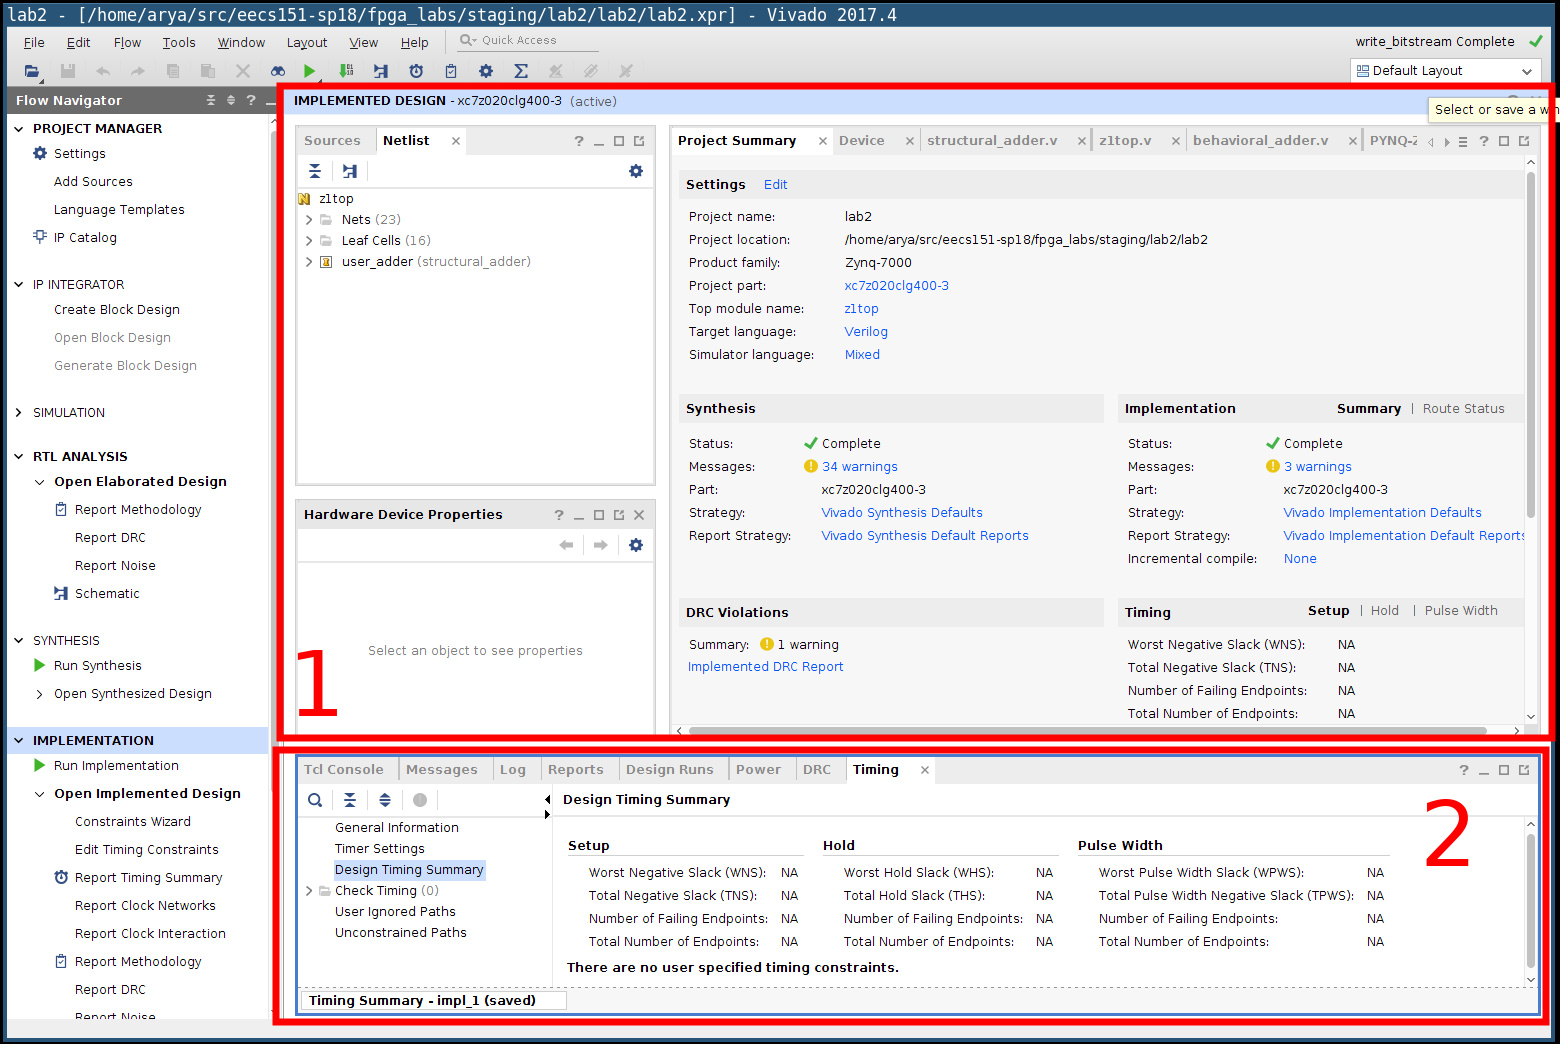
\includegraphics[width=0.7\textwidth]{figs/vivado_project_summary.png}
\end{center}

\subsection{Inspection of the Structural Adder}
\subsubsection{Schematics and FPGA Layout}
Take a look at how the Verilog you wrote mapped to the primitive components on the FPGA.
Three levels of schematic are generated for you once you've run the pipeline.
In the \emph{Flow Navigator}, you can view \emph{Schematic}s under

\begin{enumerate}
  \item \emph{RTL Analysis} $\rightarrow$ \emph{Open Elaborated Design}
  \item \emph{Synthesis} $\rightarrow$ \emph{Open Synthesized Design}
  \item \emph{Implementation} $\rightarrow$ \emph{Open Implemented Design}
\end{enumerate}

The first two will give you a fairly straightforward hierarchical block-level view of your design. You will find your circuit by drilling down into the \verb|user_adder| module (that's the name you gave the instantiation of \verb|structural_adder| in \verb|z1top_adder.v|). Check to see that your structural adder module is hooked up properly and looks sane. \textbf{Take note of the primitive blocks used in your circuit.}

In the RTL Analysis (1) you are viewing a visualisation of the topology your RTL describes. At this point, logic elaboration is very abstract: you'll notice that your logic is expressed in terms of the logic gates you described (XOR, AND, etc).
In the Synthesis schematic (2) this logic has been elaborated further into what look like FPGA elements, but still at higher layer of abstraction.
In the final schematic of the three, Implementation (3), the schematic now shows which of the elements in your nominated chip are actually targeted.

Look at how your circuit was placed and laid out on the FPGA.
Once you've run the pipeline, open \emph{Implemented Design}, click on the \emph{Window} menu, and select \emph{Device}.
You'll be presented with a layout of the FPGA package as in box 1 in the figure below.
It's hard to see with a small design, but the logic elements you've ended up using with your design will be highlighted.
You can highlight your own nets in the diagram to make it easier to find them by selecting a net or signal from the Netlist pane (\emph{Window} $\rightarrow$ \emph{Netlist}; see box 2).

\begin{center}
  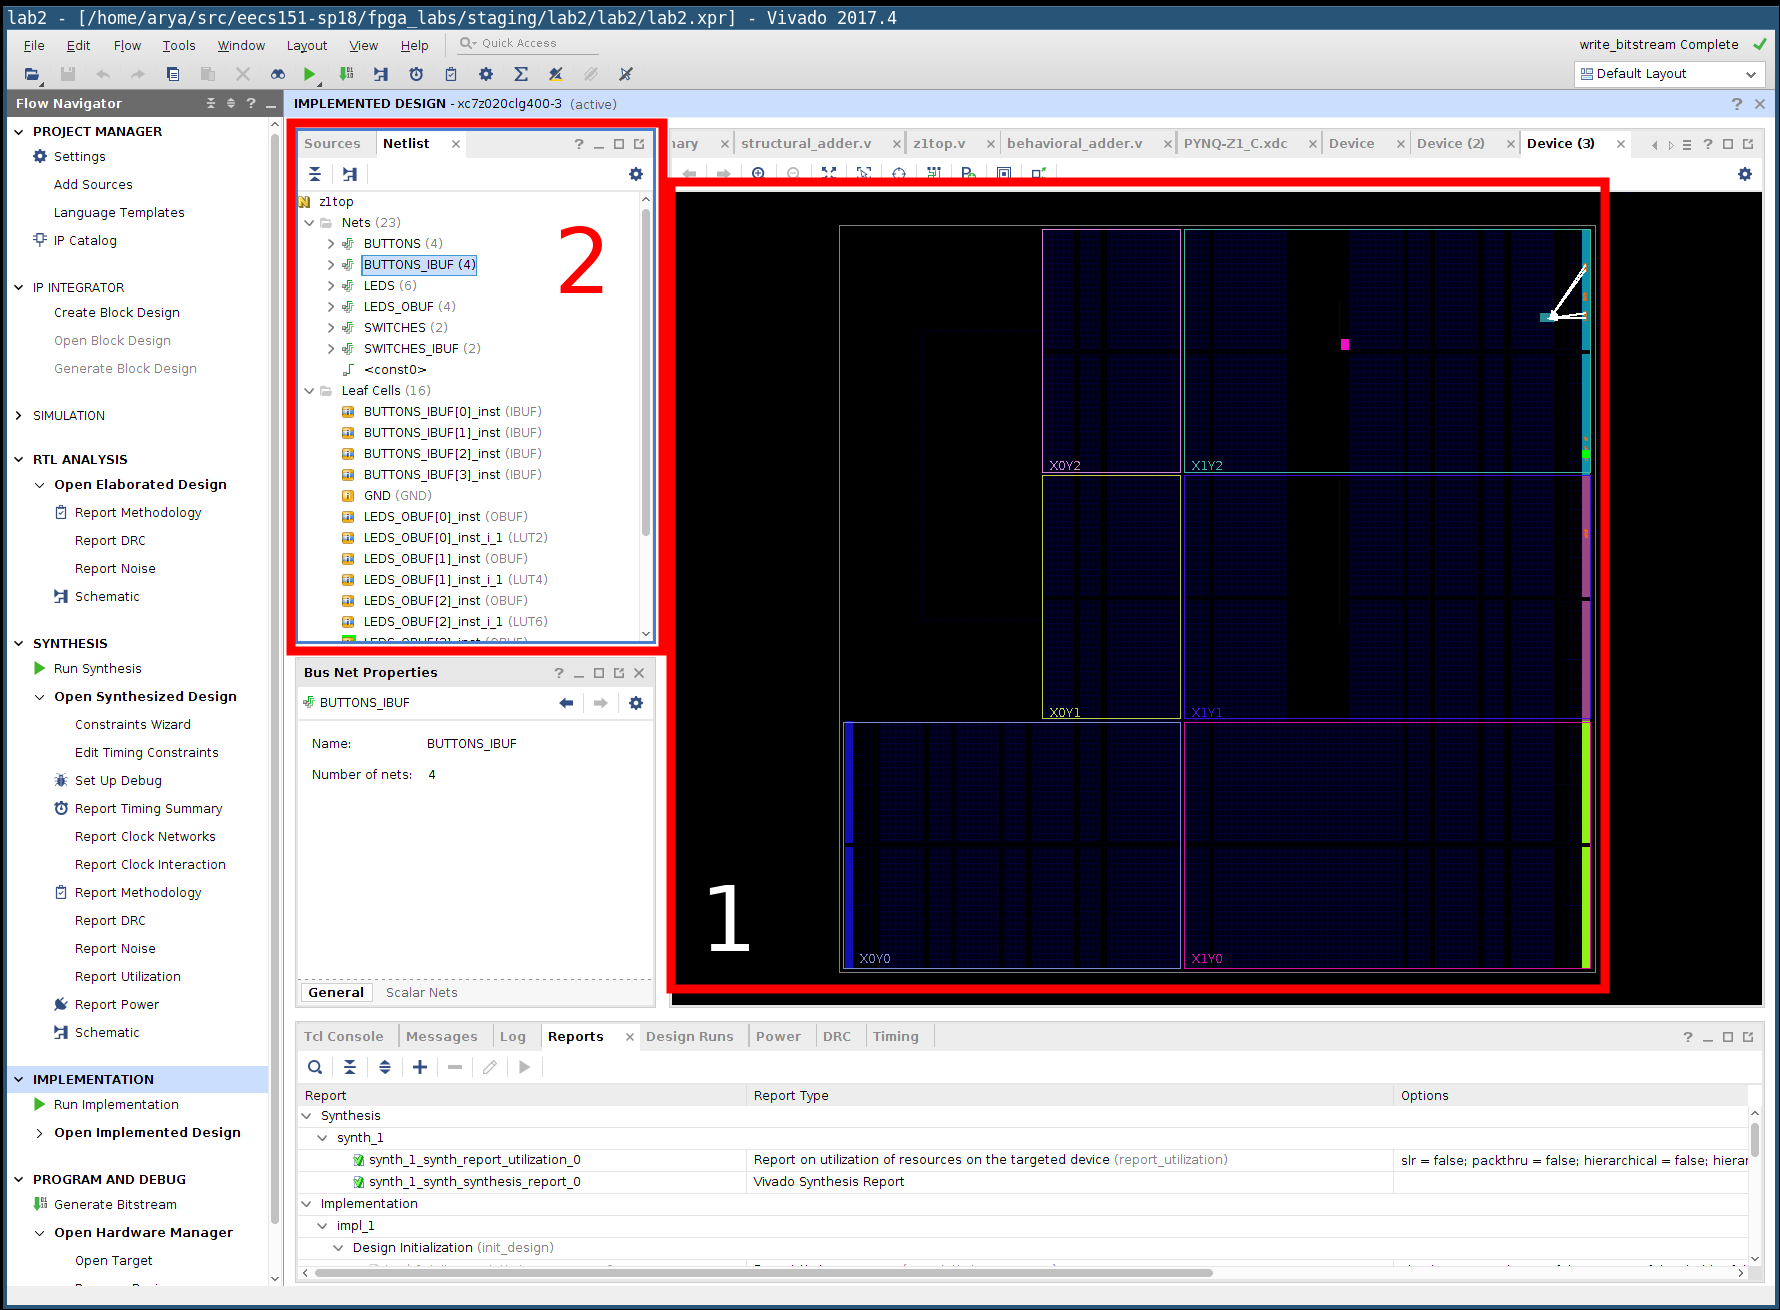
\includegraphics[width=0.7\textwidth]{figs/fpga_layout.png}
\end{center}

Explore your design and look for the modules that you wrote. If you scroll down in the \verb|Netlist Window| you should see various components of your logic. Some elements are mapped to LUTs: somewhere buried in their properties is the type of slice. See if you can find out which nets have been assigned to LUTs, and how they are connected. Go ahead and explore several SLICELs that implement the structural adder to see how they are connected to each other and the outputs of your circuit.

\subsection{Build a Behavioral 14-bit Adder}
Check out \verb|behavioral_adder.v|. It has already been filled with the appropriate logic for you. Notice how behavioral Verilog allows you to describe the function of a circuit rather than the topology or implementation.

In \verb|z1top_adder.v|, you can see that the \verb|structural_adder| and the \verb|behavioral_adder| are both instantiated in the self-test section. A module called \verb|adder_tester| has been written for you that will check that the sums generated by both your adders are equal for all possible input combinations. If both your adders are operating identically, both RGB LEDs will light up. Verify this on your board.

\subsection{Inspection of Behavioral Adder Schematics and FPGA Layout}
Go through the same steps as you did for inspecting the structural adder. View the schematics at successive levels of logic elaboration and how FPGA components are connected. Record and note down any differences you see between both types of adders in the schematic and the FPGA layouts. You will be asked for some observations in the lab report.

\section{Checkoff}
To checkoff for this lab, have these things ready to show the TA:
\begin{enumerate}
  \item Your programmed and functional board showing LED0 being controlled by BTN0 and SW0, as well as any modifications you made to the design.
  \item Demonstrate your structural adder on the FPGA and show that the test passes.
\end{enumerate}

\subsection{Lab Report}\ref{sec:labreport}
Also please submit a short lab report to gradescope in which you answer/show the following things:
\begin{enumerate}
  \item Answers for the questions in section \ref{sec:checkoffQuestions}
  \item Explain the differences between the behavioral and structural adder as they are synthesized in both the high-level schematic and low-level SLICE views
\end{enumerate}

In the next lab, we will simulate our digital designs in software, and create a \verb|tone_generator| that can play square waves through the audio jack on the Pynq board.

\section*{Ackowlegement}
This lab is the result of the work of many EECS151/251 GSIs over the years including:
\begin{itemize}
\item Sp12: James Parker, Daiwei Li, Shaoyi Cheng
\item Sp13: Shaoyi Cheng, Vincent Lee
\item Fa14: Simon Scott, Ian Juch
\item Fa15: James Martin
\item Fa16: Vighnesh Iyer
\item Fa17: George Alexandrov, Vighnesh Iyer, Nathan Narevsky
\item Sp18: Arya Reais-Parsi, Taehwan Kim
\item Fa18: Ali Moin, George Alexandrov, Andy Zhou
\item Sp19: Christopher Yarp, Arya Reais-Parsi
\end{itemize}
\end{document}
